\newpage{\ } 
\thispagestyle{empty} 

\chapter{Materiales y Metodolog\'ia}
\lhead{Capítulo 4. \emph{Materiales y Metodolog\'ia}} % This is for the header on each page - perhaps a shortened title
En este cap\'itulo se describir\'an los materiales a utilizar en la elaboraci\'on de la metodolog\'ia, como tambi\'en aquellos a utilizar en las diversas pruebas y validaciones. Ademas conoceremos las diversas caracter\'isticas que presentan las im\'agenes satelitales a ser empleados en el estudio, el cual poseen mucha relevancia debido a que constituyen variables determinantes en la elaboraci\'on de constantes al flujo de procesos.\\~\\
La metodolog\'ia nos presentara las diferentes procesos o m\'odulos necesarios, para la estimaci\'on de p\'erdida de carbono, en un marco general como tambi\'en en detalles.
\section{Materiales}
\subsection{Im\'agenes satelitales}
Los conceptos anteriores acerca de las im\'agenes sat\'elitales, nos permitir\'an describir los diferentes tipos de im\'agenes utilizados en el proyecto, de manera a brindar las caracter\'isticas relevantes en sus elecciones. 
\subsubsection{Landsat}\label{sec:landsat}
Landsat representa la colecci\'on m\'as larga y continua en el mundo de im\'agenes satelitales con resoluciones moderadas. Cuatro d\'ecadas de im\'agenes proporciona un recurso \'unico para personas que trabajan en la agricultura, geolog\'ia, silvicultura, ordenaci\'on territorial, educaci\'on, cartograf\'ia e investigaci\'on del cambio global, como tambi\'en en respuesta de emergencias y operaciones de socorro \cite{landsatNasa}.\\~\\
Las im\'agenes est\'an disponibles desde 1972 generados por una serie de 6 sat\'elites landsat. Estos sat\'elites han sido un componente importante del Programa de Observaci\'on de la tierra perteneciente a la NASA, con tres sensores primarios evolucionando a lo largo de treinta años: MSS (Multi-spectral Scanner), TM (Thematic Mapper), y ETM+ (Enhanced Thematic Mapper Plus). 
El 11 de febrero del 2013 fue lanzado el Lansadt 8 correspondiendo al futuro de los sat\'elites landsat con dos nuevo sensores, Operational Land Imager (OLI) y el Thermal Infrared Sensor (TIRS).

\begin{table}[htbp]
	\centering
	\caption{My caption}
	\label{my-label}
	\begin{tabular}{|c|c|c|c|c|c|}
		\hline
		\multirow{2}{*}{\textbf{Landsat}} & \multicolumn{5}{c|}{\textbf{Resoluciones}}                                                             \\ \cline{2-6} 
		& \textbf{Espacial} & \textbf{Espectral} & \textbf{Radiom\'etrica} & \textbf{Temporal} & \textbf{Sensor} \\ \hline
		1                                 & 79x79 m2          & 5 bandas           & 6 bits                  & 18 dias           & MSS             \\ \hline
		2                                 & 79x79 m2          & 5 bandas           & 6 bits                  & 18 dias           & MSS             \\ \hline
		3                                 & 79x79 m2          & 5 bandas           & 6 bits                  & 18 dias           & MSS             \\ \hline
		4                                 & 30x30 m2          & 7 bandas           & 8 bits                  & 16 dias           & TM              \\ \hline
		5                                 & 30x30 m2          & 7 bandas           & 8 bits                  & 16 dias           & TM              \\ \hline
		6                                 & 30x30 m2          & 8 bandas           & 8 bits                  & 16 dias           & ETM+            \\ \hline
		7                                 & 30x30 m2          & 8 bandas           & 8 bits                  & 16 dias           & ETM+            \\ \hline
		8                                 & 30x30 m2          & 9 bandas           & 12 bits                 & 16 dias           & OLI/TIRS        \\ \hline
	\end{tabular}
	\caption{Resoluciones de los sat\'elites Landsat.}
\end{table}
El Sistema de Referencia Mundial Landsat-2 (WRS-2: Landsat Worldwide Reference System-2) provee un esquema de indexaci\'on para el patr\'on de repetici\'on de la trayectoria orbital terrestre seguida por las plataformas espaciales Landsat 4, 5 y 7 sobre los 16 d\'ias de su repetitivo ciclo orbital \cite{els2015refere}. El original WRS (WRS-1) fue dise\~{n}ado para las misiones Landsat 1, 2, y 3, las cuales se movieron en una \'orbita m\'as alta. El actual WRS-2 fue dise\~{n}ado para la \'orbita a 705 Km usada para las \'ultimas misiones.

\begin{figure}[H]
	\centering
	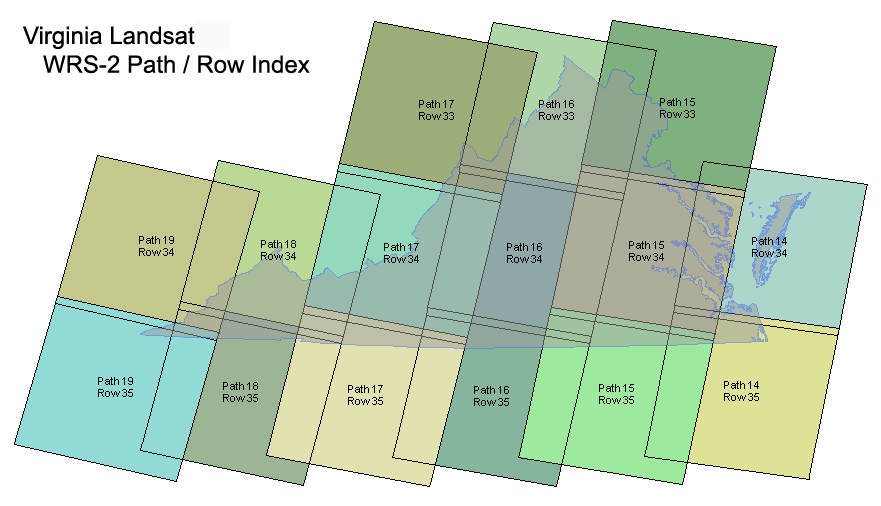
\includegraphics[width=0.8	\textwidth]{./Figures/cap4/va_wrs2b.png}
	\caption{Ejemplo WRS-2 Path/Row}
	\label{fig:wrs2Image}
\end{figure}

El Servicio Geol\'ogico de los Estados Unidos (USGS) es una agencia cientifica de los Estados Unidos, el cual proveen un producto llamado L1T (Level 1 Terrain Corrected) que implica las im\'agenes Landsat con datos pre-procesados para una precisión radiom\'etrica sistem\'atica y precisi\'on geom\'etrica mediante la incorporaci\'on de puntos de control en tierra. Estos productos est\'an en la Web de forma gratuita \cite{landsatNasa}.


\subsubsection{Vegetation Continuous Fields}\label{sec:vcf}
Las im\'agenes VCF (Vegetation Continuous Fields) contiene estimaciones proporcionales para los tipos de cobertura vegetal: vegetaci\'on le\~{n}osa, vegetaci\'on herb\'acea y suelo desnudo. El producto se deriva de las siete bandas del sensor MODerate-resolution Imaging Spectroradiometer (MODIS) a bordo del sat\'elite Terra, perteneciente a la NASA. El esquema de clasificaci\'on continuo del VCF puede representa \'areas terrestres heterog\'eneas mejor que los esquemas tradicionales de clasificaci\'on discreta. Mientras que los sistemas de clasificaci\'on tradicionales indican donde se concentran los tipos de cobertura del suelo, este producto VCF es magnifico para mostrar cuanto de cobertura forestal o pradera existe en cualquier parte de la tierra. El VCF posee un resoluci\'on espacial de 250x250 metros cuadrados y la colecci\'on de im\'agenes se encuentra disponible gratuitamente en la Web \cite{gl2015Uni}.
\begin{table}[htbp]\centering
\begin{tabular}{|c|c|}
	\hline \textbf{Valor Digital} & \textbf{Representaci\'on} \\ 
	\hline 0-100 & Porcentaje de \'area vegetal \\ 
	\hline 200 & Agua \\ 
	\hline 253 & Nulo \\ 
	\hline 
\end{tabular} 
\caption{Representaci\'on del valor digital en la imagen VCF.}
\end{table}

\begin{figure}[H]
	\centering
	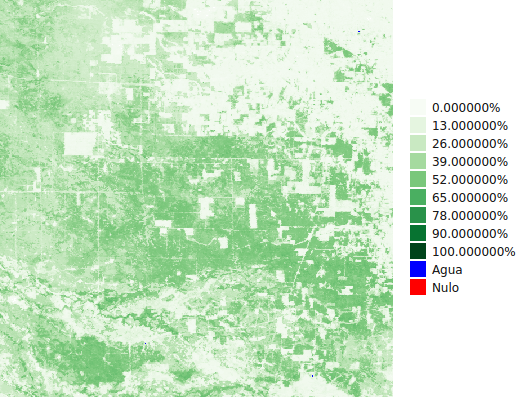
\includegraphics[width=0.8	\textwidth]{./Figures/cap4/vcf_image.png}
	\caption{Imagen VCF}
	\label{fig:vcfImage}
\end{figure}
\subsubsection{Mapa global de carbono - Paraguay}\label{sec:saatchiMapa}
En el antecedente \ref{sec:antecedente} hablamos de saatchi y su mapa global de carbono, que nos provee un promedio en toneladas de carbono por hect\'area del \'area ocupada por el pixel. Esos mapas están liberados de forma gratuita para cada pa\'is, en donde Paraguay no es la excepci\'on.
\begin{figure}[H]
	\centering
	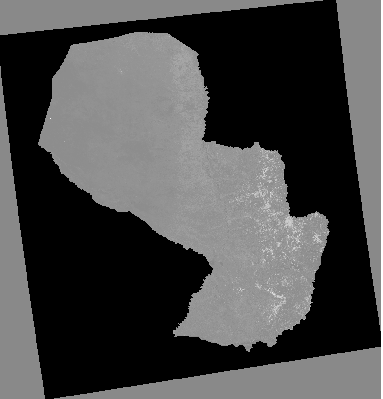
\includegraphics[width=0.8	\textwidth]{./Figures/cap5/saatchi.png}
	\caption{Mapa Global de Carbono - Paraguay}
	\label{fig:saatchi}
\end{figure}


\subsubsection{Paraguay Forest Change Product}\label{sec:fcc}
El Paraguay Forest Change Product (PFCP) muestra donde ocurri\'o la deforestaci\'on en Paraguay durante 1990-2000. El PFCP fue elaborado a partir de las im\'agenes Landsat TM y ETM+, identificando seis clases; bosque atl\'antico, Chaco bosques, el agua, no forestales y la deforestaci\'on. El producto puede ser utilizado como un ejemplo para evaluar cuantitativamente el cambio de cobertura terrestre, tambi\'en el de ayudar a determinar el proceso y el patr\'on de cambio en la cubierta forestal. La imagen se encuentra disponible gratuitamente en la Web \cite{gl2015Uni}.
\begin{table}[htbp]\centering
\begin{tabular}{|c|c|c|}
	\hline \textbf{Valor digital} &\textbf{ Representaci\'on} & \textbf{Color sugerido} \\ 
	\hline 1 & Bosque Atl\'antico & Verde \\ 
	\hline 2 & Bosque Chaque\~{n}o & Verde Claro \\ 
	\hline 3 & No Bosque & Agua \\ 
	\hline 4 & Agua & Azul \\ 
	\hline 5 & P\'erdida Bosque Atl\'antico & Rojo \\ 
	\hline 6 & P\'erdida Bosque Chaque\~{n}o & Purpura Claro \\ 
	\hline 
\end{tabular} 
\caption{Representaci\'on del valor digital en la imagen PFCP.}
\end{table}

\begin{figure}[H]
	\centering
	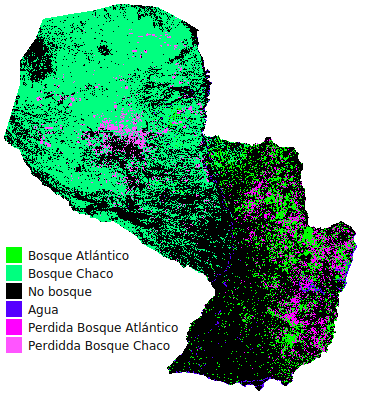
\includegraphics[width=0.7	\textwidth]{./Figures/cap4/fcc_paraguay.png}
	\caption{Paraguay Forest Change Product}
	\label{fig:fcc}
\end{figure}



\subsection{Software}
Sistemas de informaci\'on geogr\'afica fueron utilizados para la manipulaci\'on de imagenes satelitales, como tambi\'en para dise\~{n}ar e implementar los algoritmos utilizados en la metodolog\'ia propuesta.
\subsubsection{GRASS}\label{sec:grass}
GRASS es un software SIG  bajo licencia GPL (software libre). Puede soportar informaci\'on tanto raster como vectorial y posee herramientas de procesado digital de im\'agenes. Esta disponibles principalmente para plataformas Linux.
\subsubsection{Quantum GIS}\label{sec:quantum}
Quantum GIS es un SIG de c\'odigo libre para plataformas GNU/Linux, Unix, Mac OS, Microsoft Windows y Android. La principal diferencia con el GRASS es la interfaz amigable con que cuenta y la facilidad de integraci\'on con nuevas funciones espaciales desarrollados por los usuarios, esto es posible debido a que la aplicaci\'on posee un soporte muy estable para lenguajes amplios en el manejo de datos espaciales, siendo C++ y python.
\section{Metodolog\'ia}
Con los conceptos y materiales planteados en anteriores apartados, se pretende establecer una flujo de procesos o m\'odulos necesarios para el logro de los objetivos en la investigaci\'on. Se busca que los algoritmos a implementar sean ligeros en cada proceso, de manera a evitar c\'alculos complejos y excesivas supervisiones, para ello es necesario determinar comportamientos estad\'isticos de la cobertura vegetal, representados en las im\'agenes satelitales, que actuaran como variables constantes en cada proceso.\\~\\
Se plantea como datos de entrada las im\'agenes Landsat por su disponibilidad en el tiempo y gratuita obtenci\'on. Se recomienda que en el caso de utilizar imagen Landsat 8, no se mezclen im\'agenes de otro sensor del sat\'elite ya que esta posee una resoluci\'on radiom\'etrica de 16 bits y las dem\'as son capturadas a 8 bits. Por ultimo las bandas utilizadas corresponde a la infrarroja cercana y Roja.
\begin{figure}[H]
	\centering
	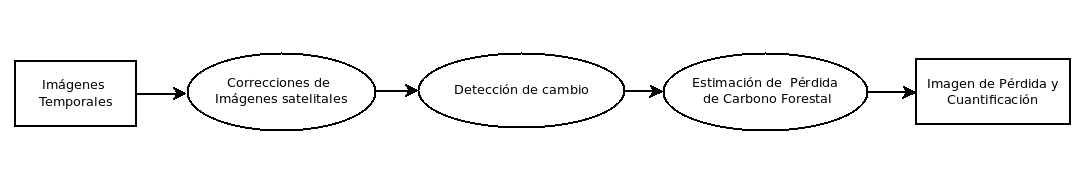
\includegraphics[width=1.0	\textwidth]{./Figures/cap4/metodologiaCarbono.png}
	\caption{Diagrama de flujo. Metodolog\'ia propuesta}
	\label{fig:metodologiapc}
\end{figure}

\subsection{Correcciones de im\'agenes satelitales}\label{sec:coorImsat}
Es necesario que los pixeles en las im\'agenes posean una ubicaci\'on suficientemente aproximada a la realidad del terreno, de manera que se garantice la correspondencia geogr\'afica entre pixeles a ser comparados. Por ello se lleva a cabo pre-procesamientos de la im\'agenes aplicando correcciones geom\'etricas y radiom\'etricas.
\subsubsection{Correcci\'on Geom\'etrica}
Este procedimiento es m\'as conocido como georeferenciaci\'on consistiendo en 3 fases; puntos de control, interpolacion espacial y radiom\'etricos \ref{sec:corrGeometrica}. Para llevar a cabo el proceso de interpolaci\'on espacial es necesario la recopilaci\'on de puntos de control, dispersos en la imagen, a trav\'es de visitas al terreno o mediante el relevamientos de datos cartogr\'aficos existentes (Mapa de caminos, ríos, cruces, etc.).
\begin{figure}[H]
	\centering
	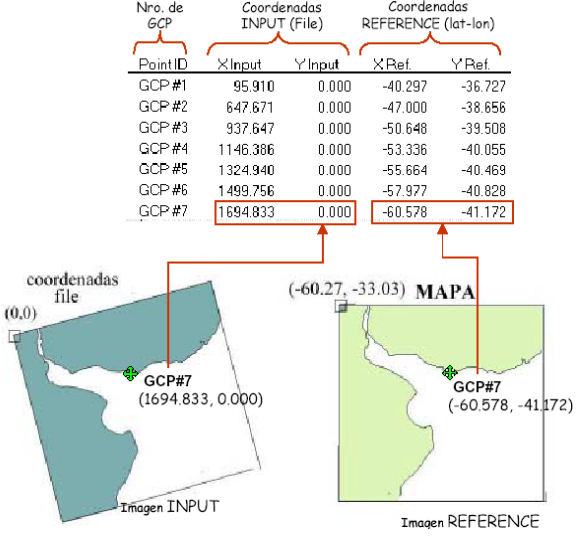
\includegraphics[width=0.7	\textwidth]{./Figures/cap4/ejGpc.png}
	\caption{Levantamiento de puntos de control.}
	\label{fig:gcp}
\end{figure}

La ecuaci\'on de transformaci\'on es una regresi\'on que relaciona los valores de coordenadas, pertenecientes a la imagen, con las coordenadas cartogr\'aficas. Los coeficientes de transformaci\'on se obtienen a partir de los puntos de control seleccionados, aplicando un ajuste por m\'inimos cuadrados de todos los puntos. Cuando la contribuci\'on de los puntos al $ RMS $ es alta, significa que las correspondencias de puntos esta mal seleccionada y que no corresponden al modelo de transformaci\'on entre la imagen y la referencia. Por ello se tiene un umbral donde los puntos que sobre pasan son borrados, re-calculando el RMS. En nuestra modelo utilizaremos 0,5 p\'ixel de la imagen, como umbral. La redundancia de datos har\'a que la bondad de ajuste tenga significaci\'on estad\'isticas y proporcione una mayor fiabilidad. La regresi\'on para esta m\'etodologia es lineal.\\~\\
La ultima fase en la correcci\'on geom\'etrica consiste en la interpolaci\'on radiom\'etrica, donde se lleva a cabo el re-muestreo de los p\'ixeles a una nueva posici\'on utilizando el m\'etodo de convoluci\'on c\'ubica, seleccionada por su mayor precisi\'on.\\~\\
A continuaci\'on los algoritmos empleados para la correcci\'on geom\'etrica:
\begin{algorithm}
	\caption{Algoritmo de correci\'on geom\'etrica}
	\label{alg:corrGEom}
	\begin{algorithmic}[1]
		\Require{Puntos de control($pc$) y las bandas de la imagen($bandas$)}
		\Statex
		\Function{correcionGeometrica}{$pc,bandas$}
		
		\State $a \gets \text{vector de coeficientes para la axisa}$
		\State $b \gets \text{vector de coeficientes para la ordenada}$
		
		\State $\textsc{coeficientesAjusteRMS}((p,a,b))$
		
		\State 
		\State $i \gets 0$
		
		\While{$bandas[i] < bandas.size$}
			\For{$x \gets 0, banda[i].filas$}
				\For{$y \gets 0, banda[i].columnas$}
					\State $\textsc{transformacion}(x,y,a,b,bandas[i],bandacorr[i])$
				\EndFor
			\EndFor
		\EndWhile
		
		\EndFunction
		
		\State
		\State
		\Procedure{transformacion}{$c,l,a,b,banda,bandacorr$}
			\State $x = a[0]+a[1].c+a[2].l$
			\State $y = b[0]+b[1].c+b[2].l$
			
			\State $bandacorr[x][y]=\textsc{convolucionCubica}(x,y,c,l,banda)$
			
		\EndProcedure
	\end{algorithmic}
\end{algorithm}


\subsubsection{Correcci\'on Radiom\'etrica}
Los bandeo y los pixeles perdidos causados por factores del sensor como ambientales, podr\'ian generar errores para la extracci\'on de informaci\'on al combinar bandas en c\'alculos de indices y variables estad\'isticas, necesarios para la discriminaci\'on de cobertura vegetal y detecci\'on de cambio. Por ello, se plantea un sub-proceso que realice la correcci\'on radiom\'etrica aplicando los m\'etodos de bandeo \ref{subsec:bandeado} y pixel o lineas perdidas \ref{subsec:pixelesP}.

\subsection{Detecci\'on de cambio forestal}
La detecci\'on de cambio cumple un papel fundamental en la metodolog\'ia, ya que nos permite categorizar el cambio en las series temporales estudiadas. Este proceso presenta un sistema automatizado a trav\'es del calculo estad\'isticas extra\'ido de las im\'agenes \ref{sec:discriminacion}, como tambi\'en de variables constantes determinadas en un previo an\'alisis del comportamiento espectral observados en la cobertura vegetal de prueba \ref{subsec:umbralVegetacion}.

\subsubsection{Detecci\'on de cambio}
La siguiente ilustraci\'on \ref{fig:deteccionCambio} presenta un panorama especifico de lo que se busca en el proceso. El resultado esperado constituye una mascara de cambio entre las series temporales de im\'agenes comparadas.
\begin{figure}[H]
	\centering
	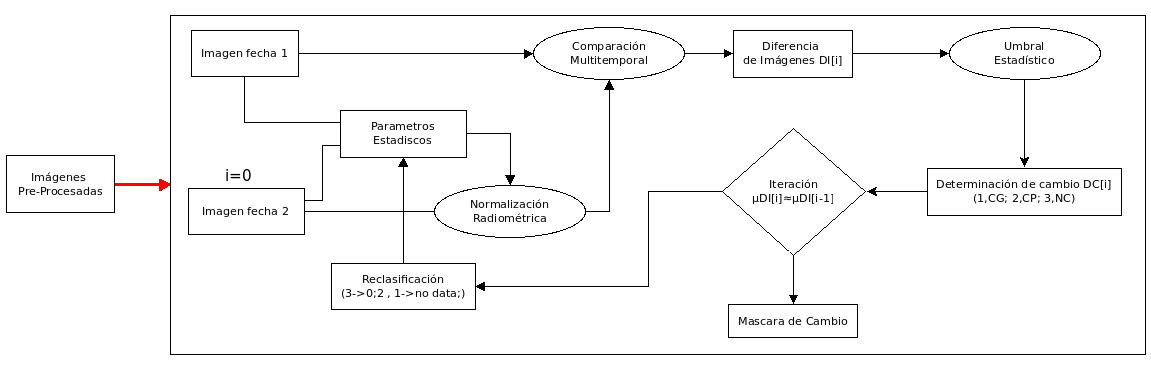
\includegraphics[width=1.0	\textwidth]{./Figures/cap4/deteccionCambio.png}
	\caption{Diagrama de flujo. Detecci\'on de Cambio.}
	\label{fig:deteccionCambio}
\end{figure}

\paragraph{Nomalizaci\'on Radiom\'etrica}\mbox{}\\\mbox{}\\
La normalizaci\'on radiom\'etrica pretende optimizar el proceso de comparaci\'on, mejorando la semejanza entre im\'agenes. Debido a la respuesta espectral que presentan las coberturas vegetales en diferentes estaciones del a\~{n}o o condiciones ambientales en el momento de la captura, es necesario un procedimiento adicional que iguale los pixeles en relaci\'on a contraste y brillo entre im\'agenes. Es un proceso similar al m\'etodo del bandeado \ref{subsec:bandeado}, empleado en la correcci\'on radiom\'etrica entre bandas de una misma imagen. Tomando como referencia los trabajo de Singh\cite{singh1989review}; Mateu y Ruiz\cite{mateu1999comparacion}; Estornell \cite{estornell2004analisis}; Mena y Malpica\cite{malpica2002fusion}, se aplicaran m\'etodos de normalizaci\'on mediante par\'ametros estad\'isticos de la imagen.\\~\\
En las distintas bandas de una imagen satelital se observan un comportamiento con distribucion normal en sus histogramas, por lo que teniendo una variable tipificada $(Z)$ es posible definirlos en una distribuci\'on normal est\'andar del tipo $ N(0,1) $ seg\'un la expresión:
	\begin{equation}
	Z=\dfrac{ND_{i}-\mu_{i}}{\sigma_{i}}
	\end{equation}
\nomenclature[56]{$ Z $}{Variable tipificada.}	
	Aplicando este concepto sobre cada una de las dos im\'agenes, se pueden comparar siendo ambas distribuciones estandarizadas:
	\begin{equation}
	\dfrac{ND_{i_{1}}-\mu_{i_{1}}}{\sigma_{i_{1}}}=\dfrac{ND_{i_{2}}-\mu_{i_{2}}}{\sigma_{i_{2}}}
	\end{equation}
	Para su aplicaci\'on pr\'actica, se puede transformar el nivel digital $ (ND_{i_{1}}) $ perteneciente a la imagen 1, para que se asemeje al $ ND_{i_{2}} $ de la imagen 2, ambas de la banda $ i $, expresi\'on:
	\begin{equation}
	ND_{i_{1}}^{'}=\mu_{i_{2}}+\dfrac{\sigma_{i_{2}}}{\sigma_{i_{1}}}\cdot(ND_{i_{1}}-\mu_{i_{1}})
	\end{equation}
	 Siendo $ ND_{i_{1}}^{'} $ la imagen normalizada. As\'i se puede definir una relaci\'on lineal entre las dos distribuciones; aplicando una normalizaci\'on radiom\'etrica estad\'istica, los coeficientes de la transformaci\'on $ m_{1,2} $ y $ h_{1,2} $ se definen seg\'un se indica en la expresi\'on:
	
			\begin{equation}
			h_{1,2}=\mu_{i_{2}}-\dfrac{\sigma_{i_{2}}}{\sigma_{i_{1}}}\cdot\mu_{i_{1}}
			\end{equation}
					\begin{equation}
					m_{1,2}=\dfrac{\sigma_{i_{2}}}{\sigma_{i_{1}}}
					\end{equation}
		\begin{equation}
				ND_{i_{1}}^{'}=m_{1,2}\cdot ND_{i_{1}}+h_{1,2}
		\end{equation}
		\nomenclature[57]{$ ND_{i_{1}}^{'} $}{Imagen normalizada, de la banda $ i $.}	
	Mediante esta transformaci\'on se obtienen histogramas parecidos, logrando de este modo mayor semejanza para el proceso de comparaci\'on multitemporal.
	
	\begin{figure}[H]
		\centering
		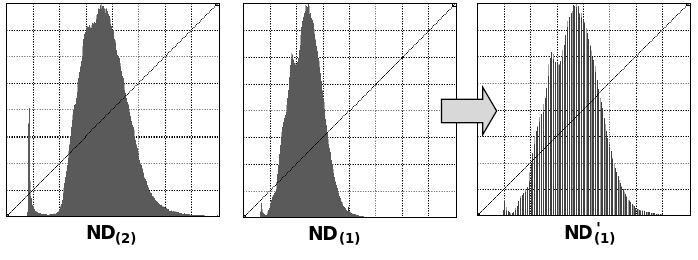
\includegraphics[width=1.0	\textwidth]{./Figures/cap4/normaRadio.png}
		\caption{Normalizaci\'on Radiom\'etrica.}
		\label{fig:normRadio}
	\end{figure}
	
	
\paragraph{Comparaci\'on Multitemporal}\mbox{}\\\mbox{}\\
Una vez equiparados radiom\'etricamente las im\'agenes, el siguiente paso consiste en la comparaci\'on multitemporal que nos permitir\'an obtener un indice de cambio (variable cuantitativa) en cada pixel resultante. Se aplicara el m\'etodo de Diferencia de im\'agenes \ref{subsec:compMult}, debido a que el m\'etodo Ratio no se ajusta a una distribuci\'on normal, condici\'on clave para la umbralizaci\'on estad\'istica. La comparaci\'on sera realizado sobre el NDVI \ref{subsec:ndvi} de cada serie temporal, a modo a resaltar la vegetaci\'on y simplificar la cantidad de bandas utilizadas, observando a su vez que los datos estables ser\'an pr\'oximos a 0, gracias a la semejanza existente entre los pixeles. 
\paragraph{Umbral estad\'istico}\mbox{}\\\mbox{}\\
Los criterios de decisi\'on propuesto en el capitulo anterior \ref{sec:discriminacion}, asignan valores de cambio/no cambio en funci\'on a un umbral, generando una mascara de cambio con valores cualitativos a partir de la imagen que contiene los $ I_{c} $, es decir, clasifica cada \'indice de cambio. Ell m\'etodo basados en par\'ametros estad\'isticos es escogido por su sencillez y coherencia con el m\'etodo de comparaci\'on multitemporal aplicada. \\~\\
La imagen es re-clasificadas en distintas categor\'ias mediante los umbrales calculados (Perdida=2, Ganancia=1, No cambio=3) y eligiendo la variable de fiabilidad $ n $ en base a la probabilidad de cambio deseado para la detecci\'on.
	\begin{figure}[H]
		\centering
		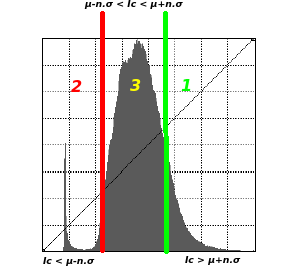
\includegraphics[width=0.7	\textwidth]{./Figures/cap4/umbrales.png}
		\caption{Umbrales y valores cualitativas asignadas en cada categor\'ia.}
		\label{fig:umbrales}
	\end{figure}

\paragraph{Iteraci\'on}\label{subsec:iteracion}\mbox{}\\\mbox{}\\
 Si dos im\'agenes se consideran semejantes, los cambios producidos en el terreno afectan a la radiometr\'ia registrada en las im\'agenes, y por tanto, en los par\'ametros estad\'isticos que las definen. En Estornell\cite{estornell2004analisis} se asume que el porcentaje de cambios existentes entre las dos im\'agenes es muy reducido.\\~\\
Se plantea la hip\'otesis, que en la normalizaci\'on radiom\'etrica los cambios introducen ruido. Cuando mayor sea la superficie de cambio, mayor sera su influencia en la normalizaci\'on y por ende la detecci\'on de cambios. En vista al problema, se pretende minimizar dicha influencia, proponiendo una normalizaci\'on radiom\'etrica iterativa, donde los par\'ametros estad\'isticos utilizados constituyen pixeles sin cambios. \\~\\
	\begin{figure}[H]
		\centering
		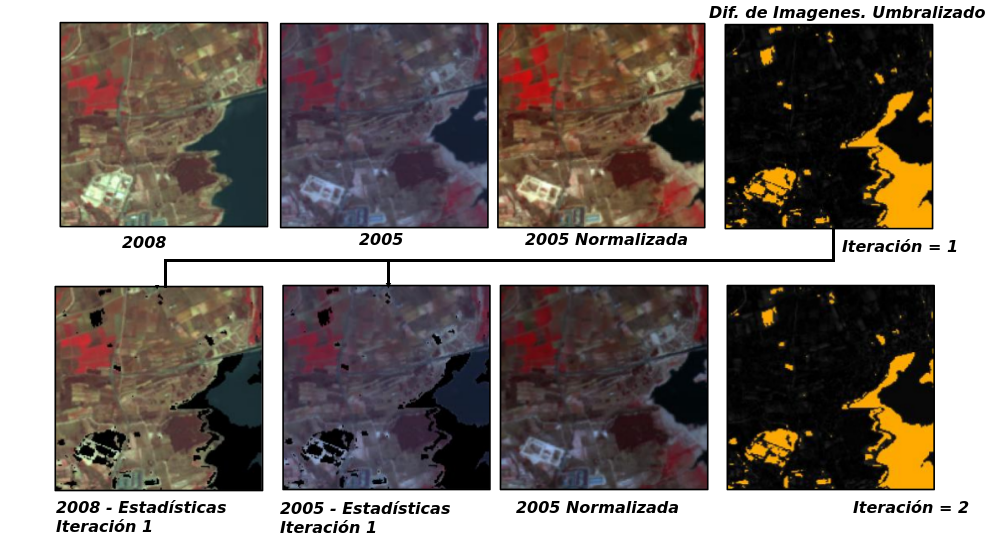
\includegraphics[width=0.7	\textwidth]{./Figures/cap4/iteracionUmbra.png}
		\caption{Mascaras de cambio, iteraci\'on de la normalizaci\'on radiom\'etrica.}
		\label{fig:umbrales}
	\end{figure}
En la m\'ascara de cambios generada por la detecci\'on de cambios, las celdas clasificadas como cambios $ (ND = 2; ND = 1) $, son re-clasificadas como $ ND=0 $; frente a las celdas de no cambio $(ND = 3)  $, clasificadas con $ ND=1 $. Esta m\'ascara re-clasificada se utiliza para suprimir los cambios de las im\'agenes radiom\'etricas utilizadas como referencia estad\'istica. El procedimiento anterior se aplica \'unicamente para estimar los par\'ametros de normalizaci\'on radiom\'etrica. La imagen sobre la que se aplica la normalizaci\'on ha de mantener todas las celdas, independientemente de que se consideren como cambios a priori. Se propone repetir las iteraciones hasta que la media de las diferencias entre NDVI, sea de magnitud similar a la media obtenida en la iteraci\'on anterior. 
\begin{algorithm}
	\caption{Algoritmo de iteraci\'on}
	\label{alg:iteracionAlg}
	\begin{algorithmic}[1]
	\Statex
	
	\State $ bandaf1 \gets \text{imagen de la fecha 1} $ 
	\State $ bandaf2 \gets \text{imagen de la fecha 2} $ 
	\State $ mascCambio \gets \text{mascara de cambio} $ 
	\State $ bandaNorm \gets \text{imagen normalizada} $ 
	\State $ bandera = 0$

	
	\State 
	\State $ continuar = 1 $ 
	\State $ primera = 1 $ 
	\While{$continuar = 1$}
			\State $ mascCambio = \textsc{normalizar}(mascCambio,bandaf1,bandaf2,bandaNorm)$ 
			\If{$primera = 1 \text{ or } bandaNorm.media <> bandera$}
				\State $ continuar = 1 $ 
				\State $ primera = 0 $ 
				\State $ bandera = bandaNorm.media $
			\Else
				\State $continuar = 0$
			\EndIf
	\EndWhile
	
	\end{algorithmic}
\end{algorithm}


\subsubsection{Discriminaci\'on Forestal}
La siguiente ilustraci\'on \ref{fig:discrimForestal} refleja los pasos realizados para obtener una mascara de vegetaci\'on. Dicha m\'ascara representa si un pixel es o fue vegetaci\'on forestal en la serie temporal comparada. Los im\'agenes de entrada que ser\'an procesadas, son aquellas obtenidas en la ultima normalizaci\'on radiom\'etrica generada por el proceso de detecci\'on de cambio, como tambi\'en la imagen utilizada de referencia en ese proceso.
\begin{figure}[H]
	\centering
	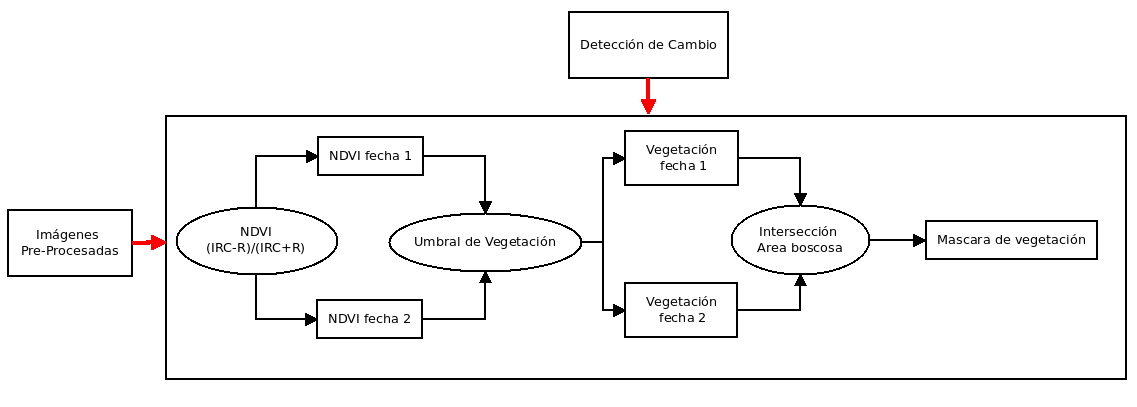
\includegraphics[width=1.0	\textwidth]{./Figures/cap4/discriminacionForestal.png}
	\caption{Diagrama de flujo. Discriminaci\'on Forestal.}
	\label{fig:discrimForestal}
\end{figure}

\paragraph{NDVI}\mbox{}\\\mbox{}\\
El NDVI es calculado para ambas fechas pertenecientes a la serie temporal evaluada. El calculo es hecho teniendo como entradas las bandas infrarroja cercana y roja, donde el vigor vegetal de cada p\'ixel sera determinado por la ecuaci\'on \ref{e:ndvi}. En total son consumidas 4 im\'agenes para obtener dos de salidas.
\paragraph{Umbral de Vegetaci\'on}\label{sec:uvegetacion}\mbox{}\\\mbox{}\\
El umbral discriminatorio para la vegetaci\'on es determinado a partir de una constante calculada por un previo estudio del comportamiento espectral de la cobertura vegetal y las im\'agenes NDVI \ref{subsec:umbralVegetacion}. Dicha variable corresponde a la desviaci\'on $(\sigma_{c} = 0.0658242733)  $ observada en el an\'alisis hecho por cruzamientos de datos entre im\'agenes VCF y Landsat. La ecuaci\'on del umbral $ U_{NDVI} $ tiene la siguiente expresi\'on:
		\begin{equation}
		U_{NDVI} = \mu_{NDVI}\pm n \sigma_{c}
		\end{equation}
\nomenclature[58]{$ \sigma_{c} $}{Desviaci\'on determinada como constante para la umbralizaci\'on de la cobertura vegetal.}
Donde $ \mu_{NDVI} $ representa la media del NDVI calculada y $ n $ la fiabilidad. No se utiliza la ecuaci\'on correspondiente a la suma, debido a que se pretende incluir \'indices por debajo de la media.
\begin{figure}[H]
	\centering
	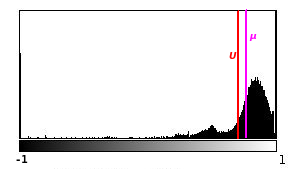
\includegraphics[width=0.8	\textwidth]{./Figures/cap4/ndviUmbral.png}
	\caption{Umbral NDVI. U=0,78076712 para n=1.}
	\label{fig:ndviUmbral}
\end{figure}

\paragraph{Intersecci\'on \'area boscosa }\mbox{}\\\mbox{}\\
Una vez obtenido la mascara de vegetaci\'on de las dos fechas, es necesario determinar las celdas que ser\'an evaluados el cambio, por ello aplicamos una simple operaci\'on de intersecci\'on que generara una mascara de vegetaci\'on para los dos tiempos.

\subsubsection{Mascara de P\'erdida Forestal}
Este proceso constituye la ultima fase, consistiendo en la intersecci\'on entre mascaras de vegetaci\'on y cambio, utilizando solo aquellos pixeles que representan perdida, para generar una imagen binaria de perdida de vegetaci\'on Forestal.\\~\\
La imagen final de cambios, independiente del método que se utilice, probablemente tendrá errores que son inherentes a los procesos utilizados para su creación \cite{lovell2001filtering}. \\~\\
Para reducir el porcentaje de falsas alarmas, se propone la utilización del filtro de mediana \ref{subsec:filMediana} sobre la imagen de perdida, como m\'etodo de eliminación de ruido. Al trabajar con im\'agenes de media/alta resoluci\'on espacial(menos de 15x15 metros cuadrados), se obtienen buenos resultados aplicando filtros de 5x5; pero cuando se trabaje con im\'agenes de menor resoluci\'on no se recomienda ese tama\~{n}o de ventana por la distorsi\'on que causa a la imagen \cite{martinez2013normalizacion}. Nuestras im\'agenes satelitales de entrada son de baja resoluci\'on espacial (30x30 metros cuadrados) por lo que el tama\~{n}o de ventana a utilizar seria 3x3.
La siguiente ilustraci\'on representa el flujo de tareas \ref{fig:intersPerdida}.
\begin{figure}[H]
	\centering
	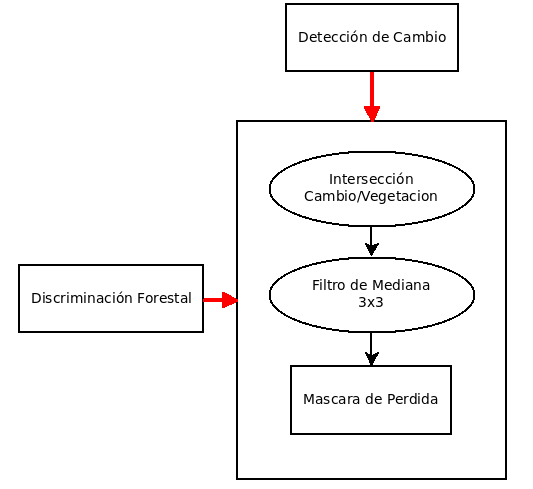
\includegraphics[width=0.8	\textwidth]{./Figures/cap4/interseccionPerdida.png}
	\caption{Diagrama de flujo. Mascara P\'erdida Forestal.}
	\label{fig:intersPerdida}
\end{figure}

\subsection{Estimaci\'on de p\'erdida de carbono forestal}
El procedimiento final consiste en estimar el carbono perdido o no secuestrados dentro del tiempo transcurrido entre las im\'agenes satelitales. El producto constituye la mascara de perdida forestal junto con la cuantificaci\'on en toneladas de carbono por hect\'area, obtenida mediante la ecuaci\'on de regresi\'on lineal $(y= b + ax) $ que fue generada a través del mapa global de carbono \cite{saatchi2011benchmark} y el NDVI, determinadas por las im\'agenes Landsat, en un estudio previo \ref{subsec:estimacionCarbono}. La regresi\'on presenta un coeficiente de determinaci\'on $ (r^{2}=0.509125) $ moderado, según tabla \ref{t:coefDeter}, por lo que el estudio es considerado valido para su aplicaci\'on en la metodolog\'ia.
\nomenclature[59]{$ r^{2}$}{Coeficiente de determinaci\'on.}
\begin{table}[H]
	\centering
	\begin{tabular}{|l|l|}
		\hline
		\textbf{Valor} & \textbf{Significado} \\ \hline
		0,0            & Ninguna Relaci\'on     \\ \hline
		0,25           & Relaci\'on baja        \\ \hline
		0,50           & Relaci\'on Moderada    \\ \hline
		0,75           & Relaci\'on Buena       \\ \hline
		1,00           & Relaci\'on perfecta    \\ \hline
	\end{tabular}
	\caption{Rangos del coeficiente de determinaci\'on.}
	\label{t:coefDeter}
\end{table}
Sea $ C:(x,y) \longrightarrow \{ [-\infty,\infty]\}$ la cantidad de carbono, en toneladas por hect\'area, para la coordenada $ (x,y) $, se tiene que: 

		\begin{equation}
			C(x,y)=4,33+30,1 ndvi(x,y)
		\end{equation}
		\nomenclature[60]{$ C(x,y)$}{Toneladas de carbono por hect\'area en las coordenadas $ (x,y) $.}


 Para no realizar el calculo de carbono repetidamente en cada imagen de la secuencia temporal y luego restarlas con finalidad de tener la perdida producida en los p\'ixeles, se optimizo el proceso  utilizando la imagen con indices de cambios resultante $ (Ic) $ del proceso de iteraci\'on \ref{subsec:iteracion}, por lo que la ecuaci\'on quedara modificada con las siguientes expresiones para dos fechas {}:
		\begin{equation}
				\label{e:fecha1}
		C(x_{1},y_{1})=4,33+30,1 ndvi(x_{1},y_{1})
		\end{equation}
		\begin{equation}
						\label{e:fecha2}
		C(x_{2},y_{2})=4,33+30,1 ndvi(x_{2},y_{2})
		\end{equation}
		\begin{equation}
		\label{e:indiceCambio}
		Ic(x,y)=ndvi(x_{2},y_{2}) -ndvi(x_{1},y_{1})
		\end{equation}		
Restando el carbono obtenido entre cada fecha, ecuación \ref{e:fecha2} y \ref{e:fecha1}, tendr\'iamos:
		\begin{equation}
				\label{e:restaCar}
		C(x_{2},y_{2}) - C(x_{1},y_{1})= 30,1(ndvi(x_{2},y_{2})-ndvi(x_{1},y_{1}))
		\end{equation}		
				\begin{equation}
				\label{e:perdidaCar}
					PC(x,y)= C(x_{2},y_{2}) - C(x_{1},y_{1})
				\end{equation}		
\nomenclature[62]{$Ic(x,y)$}{ Indice de cambio en las coordenadas $ (x,y) $.}
\nomenclature[63]{$PC(x,y)$}{Toneladas de carbono por hect\'area perdidos en las coordenadas $ (x,y) $.}
Siendo $ PC(x,y)$ Toneladas de carbono por hect\'area perdidos. Remplazando \ref{e:indiceCambio} y \ref{e:perdidaCar} en \ref{e:restaCar}, la ecuaci\'on de regresi\'on final quedar\'ia:
		\begin{equation}
			PC(x,y) = 30,1 Ic(x,y)
		\end{equation}
La cuantificaci\'on sera realizado teniendo en cuenta la mascara de perdida forestal.
\begin{figure}[H]
	\centering
	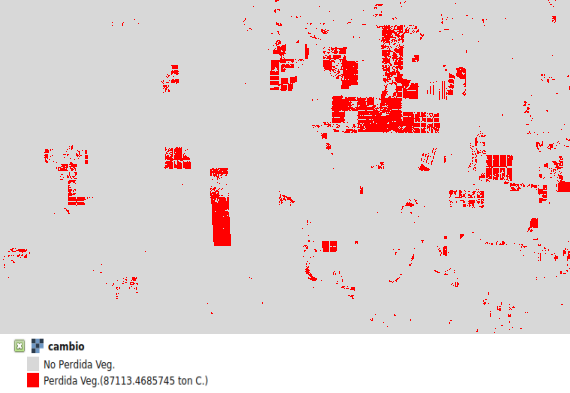
\includegraphics[width=0.8	\textwidth]{./Figures/cap4/resultadoMetodologia.png}
	\caption{Presentaci\'on del resultado. Mascara de perdida Vegetal y cuantificaci\'on.}
	\label{fig:resulPC}
\end{figure}
\section{Resumen}
En este capitulo se describen los materiales y los tres procedimientos generales que componen la metodolog\'ia propuesta. La im\'agenes infrarroja cercana y roja de las dos fechas inicialmente deben pasar por un proceso de correcci\'on de errores del sensor y de ubicaci\'on geogr\'afica para realizar el an\'alisis multitemporal en la detecci\'on de cambio forestal. Una vez detectado la perdida forestal entre las fechas del proceso de detecci\'on de cambio, se realiza la estimaci\'on de carbono en base a una ecuaci\'on de regresi\'on hallado por un estudio previo. El resultado consiste en un mapa de perdida forestal junto a la cuantificaci\'on en toneladas de carbono perdidos.